% Note that the text in the [] brackets is the one that will
% appear in the table of contents, whilst the text in the {}
% brackets will appear in the main thesis.

%% CHAPTER HEADER /////////////////////////////////////////////////////////////////////////////////////
\chapter{Experimental Validation of the Models}
\label{ch:validation}

%% CHAPTER INTRODUCTION ///////////////////////////////////////////////////////////////////////////////
The Chapter includes an assessment of the accuracy and reliability of the modelled physical processes.
In order to validate the sensor model, in the frequency-domain \ac{emi} characteristic was determined through numerical simulations.
The characteristic was then compared with values obtained by theoretical analysis and with experimental measurements.
On the other hand, \ac{hsc} panel model was evaluated experimentally in two ways: by analysing the full wavefield obtained by the \ac{sldv} and by studying the time signals measured by the \acp{pzt} setup.
%% INCLUDE SECTIONS ///////////////////////////////////////////////////////////////////////////////////
%% SECTION HEADER /////////////////////////////////////////////////////////////////////////////////////
\section{Analytical validation of the \ac{pzt} model}
\label{sec:pztVal}

%% SECTION CONTENT ////////////////////////////////////////////////////////////////////////////////////
The current model, i.e. the boundary geometry modelled with the second order elements, is validated by comparing the transducer impedance obtained by numerical simulation and analytical model derived by Giurgiutiu \cite{giurgiutiu2009micromechatronics}.
The impedance Z is a ratio between voltage \((\Phi)\) and current \((I)\) defined as follows:
\begin{eqnarray}
	Z = \frac{\Phi}{I} = \frac{\Phi}{i\omega Q},
\end{eqnarray}
where \(i=\sqrt{-1}\), \(\omega\) is the angular frequency.
In the case of numerical simulation, \(\Phi\) is assumed as the 1.5-cycle Hann windowed sine pulse, and \(Q\) is the charge induced on the electrode calculated by Equation \ref{eq:pzt_sem}. 
The excitation signal has significant values in the 0-300 kHz frequency range, as shown in Fig.~\ref{fig:impedance}(\textbf{a}).
The analytical model is defined as:
\begin{eqnarray}
	Z = \frac{1}{i\omega C_0}\left[\left(1-k_p^2\right)+k_p^2\frac{u_r}{u_I}\right],
\end{eqnarray}
where \(C_0\) is the free capacitance of the sensor, \(k_p\) is the planar coupling coefficient, \(u_r\) is the displacement response, and \(u_I\) is the induced displacement.
Additional, for the comparison, the response of the \ac{sem} with boundary approximation by linear elements was included. 
\begin{figure}[H]
	\begin{center}
		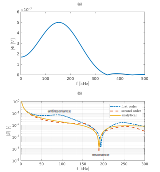
\includegraphics{Chapter_6/impedance}
	\end{center}
	\caption{Validation of the \ac{pzt} model (\textbf{a}) the frequency spectrum of the excitation signal, (\textbf{b}) impedance response of the transducer.}
	\label{fig:impedance}
\end{figure}

It can be notice in Fig.~\ref{fig:impedance}(\textbf{b}) the impedance of the current model is in very good agreement with the analytical solution.
The resonant peak occurred near 190 kHz in both cases, while the resonance of the first-order elements model is shifted 12 kHz toward the higher frequency.
In addition, an antiresonance peak occurred around 90 kHz, not observed in the previous two models.

%% SECTION HEADER /////////////////////////////////////////////////////////////////////////////////////
\section{Experimental setup for the \acs{hsc} model validation}
\label{sec:setup}
%% SECTION CONTENT ////////////////////////////////////////////////////////////////////////////////////
\begin{figure}
	\begin{center}
		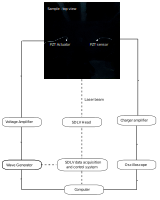
\includegraphics[width=0.95\textwidth]{Chapter_6/setup}
	\end{center}
	\caption{Experimental setup for (1) the \acf{sldv} measurement - dashed line and (2) the \acf{pzt} wave acquisition - solid line.}
	\label{fig:setup}
\end{figure}
The presented model of the \ac{hsc} was validated with results from two experimental studies.
The first one was performed for determination of the full wavefield of the propagating waves by the \ac{sldv} (Polytec PSV–400).
The second study was performed for wave acquisition by the \ac{pzt} sensor.
A schematic of the experimental scenarios is shown in Fig.~\ref{fig:setup}.

The \ac{sldv} is a modern method for non-contact measurement of the vibration velocity of structure surface particles.
The principle of vibrometer operation is based on the Doppler effect, recording the change of frequency of the light beam reflected from the vibrating surface.
In laser vibrometry, the measurement of frequency change is realised by interferometer and analysis of both reference and measurement light beam.
The measuring system is additionally equipped with mirrors allowing to change the angle of the measuring beam, so it is possible to take measurements at a grid of points on a surface of inspected structural element automatically.
The \ac{sldv} setup is presented in Fig.~\ref{fig:sldv}.
\begin{figure}
	\begin{center}
		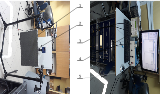
\includegraphics[width=0.95\textwidth]{Chapter_6/sldv}
	\end{center}
	\caption{The \acf{sldv} setup: 1 - the laser sensor head, 2 - the \acf{hsc} specimen, 3 - the arbitrary waveform generator, 4 - the amplifier, 5 - data management system}
	\label{fig:sldv}
\end{figure}

The \ac{pzt} elastic wave generation and acquisition system is used to measure the voltage changes of transducers due to their mechanical deformation.
It is a point measurement at the point of sensor placement.
The following instruments are required to make the measurements: waveform generator to prepare signal, amplifier to strengthen the excitation and recording signals, oscilloscope and central management unit.
The setup used for measurements is shown in Fig.~\ref{fig:pzt_setup}.
\begin{figure}[t]
	\begin{center}
		\includegraphics[width=0.95\textwidth]{Chapter_6/pzt_setup}
	\end{center}
	\caption{The \acf{pzt} setup,(\textbf{a}) elastic wave generation and acquisition instruments:  1 - data management unit - arbitrary wave generator, 2 - oscilloscope - amplifier, 3 , 4 , (\textbf{b}) the specimen held in the environmental chamber.}
	\label{fig:pzt_setup}
\end{figure}

Both methods have some advantages and disadvantages, which are given in the Table~\ref{tab:method_comp}.
\begin{table}[H]
	\small
	\tabcolsep=0.25cm
	%\centering
	\caption{\label{tab:method_comp}Comparison of methods for elastic wave propagation measurements.}
	\begin{tabular}{p{0.1\textwidth}>{\raggedright}p{0.4\textwidth}>{\raggedright \arraybackslash}p{0.4\textwidth}}
		\toprule
		\textbf{Method} &\textbf{Advantages} & \textbf{Disadvantages}\\
		\midrule
		\multirow{5}{*}{\ac{sldv}}   & \tabitem automatic full-field scanning & \tabitem high-cost equipment\\ 
		& \tabitem non-contact measurement & \tabitem long measurement time\\
		& \tabitem \ac{3d} velocity vector (optional)& \tabitem special surface treatment is needed to avoid scattering of the laser beam, e.g. by application of retroreflective tape\\
		& & \tabitem high signal-to-noise ratio\\
		& & \tabitem relatively large space need for measurements \\
		& & \tabitem special sample mounting for repeatability of measurements\\
		\midrule
		\multirow{5}{*}{\ac{pzt}} & \tabitem low-cost instruments & \tabitem spot measurement\\
		& \tabitem high repeatability of measurements & \tabitem displacements vector correlated with the sensor polarization\\
		& \tabitem measurements on the sample in motion & \tabitem cumbersome wiring\\
		& \tabitem generation and recording signals with the same setup & \tabitem sensitive to electric and magnetic fields\\		
		\bottomrule
	\end{tabular}
\end{table}

The sample was fabricated under workshop conditions from the components described in Section~\ref{sec:sample}.
Before applying the two-ingredient glue (Loctite EA3479B), the bottom surface of the skin was cleaned and degreased with the solvent (Loctite SF7063).
The adhesive curing took 48 hours under a distributed load at ambient temperature.

The subject of the parametric study was the effect of the disbond size on the propagating \ac{gw}.
After a reference measurement was made on an intact sample, several measurements were taken for the subsequent damage introduced on the same specimen.
The damage width varied in range \(\mathrm{w_d}=\left [10, 30, 50, 70, 100, 120 \right ]\) \unit{\mm}, while its fixed length was \(\mathrm{l_d} = 175\) \unit{\mm}.

The \(N_c=5\) cycle Hann windowed signal at carrier frequencies \(f_c=[50,100,150]\) \unit{\kHz} was generated using an arbitrary waveform generator (National Instruments, PXI 5413).
The signal was amplified 3.5 times and supplied to the \ac{pzt} actuator (Noliac, NCE51) by the emission/reception unit (LWDS, Cedrat Technologies).
Each measurement was conducted under a temperature of 20\unit{\degreeCelsius} controlled in the environmental chamber (DM 600C, Angelantoni Test Technologies Srl) and averaged 20~times to improve the signal-to-noise ratio.
%% SECTION HEADER /////////////////////////////////////////////////////////////////////////////////////
\section{Results of the \acs{hsc} validation with \acs{sldv} setup}
\label{sec:resuls_sldv}
%% SECTION CONTENT ////////////////////////////////////////////////////////////////////////////////////
The full wavefield in the healthy sample is presented in Fig.~\ref{fig:fullfield_50_0}, Fig.~\ref{fig:fullfield_100_0} and Fig.~\ref{fig:fullfield_150_0}.
The experimental measurements and the \ac{fcgm} snapshots show that the wavefront distortion is rising with the frequency.
Because the wavelength decreases as the frequency increases, a higher frequency signal is more likely to induce wave reflections from the core walls.
This effect can not be observed in the case of the \ac{hcgm}.

\begin{figure}[!hbt]
	\begin{center}
		\includegraphics[width=0.95\textwidth]{Chapter_6/fullfield_50_0}
	\end{center}
	\caption{The top surface out of plane particle velocity snapshots for \textbf{(a)} the \acf{fcgm}, \textbf{(b)} the experimental results obtained by using the \acf{sldv}, and \textbf{(c)} the \acf{hcgm} in the \textbf{healthy~sample at 50 kHz}.}
	\label{fig:fullfield_50_0}
\end{figure}
\begin{figure}[!hbt]
	\begin{center}
		\includegraphics[width=0.95\textwidth]{Chapter_6/fullfield_100_0}
	\end{center}
	\caption{The top surface out of plane particle velocity snapshots for \textbf{(a)} the \acf{fcgm}, \textbf{(b)} the experimental results obtained by using the \acf{sldv}, and \textbf{(c)} the \acf{hcgm} in the \textbf{healthy~sample at 100 kHz}.}
	\label{fig:fullfield_100_0}
\end{figure}
\begin{figure}[!hbt]
	\begin{center}
		\includegraphics[width=0.95\textwidth]{Chapter_6/fullfield_150_0}
	\end{center}
	\caption{The top surface out of plane particle velocity snapshots for \textbf{(a)} the \acf{fcgm}, \textbf{(b)} the experimental results obtained by using the \acf{sldv}, and \textbf{(c)} the \acf{hcgm} in the \textbf{healthy~sample at 150 kHz}.}
	\label{fig:fullfield_150_0}
\end{figure}

In case of the damaged sample, the wavefront is not distorted in the damage area bounded by dashed white rectangle in Fig.~\ref{fig:fullfield_50_5}, Fig.~\ref{fig:fullfield_100_5} and Fig.~\ref{fig:fullfield_150_5} for all three cases.
Due to the lack of wave leakage into the core, the wave propagates smoothly through the skin.
For the experimental sample and the \ac{fcgm}, interference of waves reflected from the cells and the damage boundary is observed.
The wave interference observed in the \ac{hcgm} refers to waves reflected only from the defect.

\begin{figure}[!hbt]
	\begin{center}
		\includegraphics[width=0.95\textwidth]{Chapter_6/fullfield_50_5}
	\end{center}
	\caption{The top surface out of plane particle velocity snapshots for \textbf{(a)} the \acf{fcgm}, \textbf{(b)} the experimental results obtained by using the \acf{sldv}, and \textbf{(c)} the \acf{hcgm} \textbf{with removed core elements at 50 kHz} in damaged area for both numerical models.}
	\label{fig:fullfield_50_5}
\end{figure}
\begin{figure}[!hbt]
	\begin{center}
		\includegraphics[width=0.95\textwidth]{Chapter_6/fullfield_100_5}
	\end{center}
	\caption{The top surface out of plane particle velocity snapshots for \textbf{(a)} the \acf{fcgm}, \textbf{(b)} the experimental results obtained by using the \acf{sldv}, and \textbf{(c)} the \acf{hcgm} \textbf{with removed core elements at 100 kHz} in damaged area for both numerical models.}
	\label{fig:fullfield_100_5}
\end{figure}
\begin{figure}[!hbt]
	\begin{center}
		\includegraphics[width=0.95\textwidth]{Chapter_6/fullfield_150_5}
	\end{center}
	\caption{The top surface out of plane particle velocity snapshots for \textbf{(a)} the \acf{fcgm}, \textbf{(b)} the experimental results obtained by using the \acf{sldv}, and \textbf{(c)} the \acf{hcgm} \textbf{with removed core elements at 150 kHz} in damaged area for both numerical models.}
	\label{fig:fullfield_150_5}
\end{figure}
\clearpage
\input{Chapters/Chapter6/sec:results_pzt}

\section{Conclusions}
\label{sec:conclusionsValid}

%% SECTION CONTENT ////////////////////////////////////////////////////////////////////////////////////
The Chapter presents the validation of the developed models.
The \ac{emi} characteristic of the \ac{pzt} model was in good agreement with analytically obtained characteristic and with experimental results in the analysed frequency range of 0-300 \unit{\kHz}.
The \ac{sldv} analysis showed that \ac{fcgm} expresses better wave propagation behaviour in \ac{hsc} than homogenised model.
The snapshots of the full wavefield showed wave interference in the core cells, which was impossible to obtain in the \ac{hcgm}.
The full-field analysis also showed a lack of wave leakage into the core at the damaged area.
This phenomenon is the basis for determining the effect of the damage on wave propagation.
The velocity of the wave propagation for both models was in good agreement with the \ac{pzt} measurements.